\documentclass[10pt]{article}
\usepackage{mathtools}
\usepackage{amsmath}
\usepackage{tabularx}
\usepackage{graphicx}
\usepackage{flexisym}
\usepackage{listings}
\usepackage[most]{tcolorbox}
\usepackage{xcolor}
\usepackage{hyperref}
\usepackage{amsthm}
\usepackage{subcaption}
\newtcblisting[auto counter]{pseudolisting}[2][]{sharp corners,
    fonttitle=\bfseries, colframe=gray, listing only,
    listing options={basicstyle=\ttfamily,language=c++},
    title=Listing \thetcbcounter: #2, #1}
\newtheorem*{theorem}{Theorem}

\begin{document}
\setlength\parindent{1pt}
\title{Quantum Monte Carlo of confined electrons }
\author{Andrei Kukharenka and Anna Gribkovskaya \\  
FYS 4150 
}

\maketitle
\begin{abstract}
Aim of this work is to determine the ground state energy of the quantum system using Variational Monte Carlo (VMC) method. The considered system is two electrons confined in quantum dot. Quantum dot is approximated with a three-dimensional harmonic oscillator potential. Apart of ground state energy the relative distance between two electrons and expectation values of the kinetic and potential energies were evaluated. Obtained results are compared with those obtained in second project\cite{proj2} and analytical results from Taut \cite{three}. 
\end{abstract}
\clearpage 


\section{Introduction}
System under consideration is a three-dimensional harmonic oscillator potential with two electrons. Such potential traps electrons inside and prevent them to move apart. Such systems are called quantum dots and have a large application in science \cite{four}, industry\cite{five} and medicine \cite{med}. \\
We already study such system in project two \cite{proj2} emploing brute-force approach -- using the eigenvalue solver, so we are able to compare results from different methods. The advantage of VMC method is that we can use Cartesian coordinates and do not need to transform the equations. \\ 
VMC is a method for solving Schr\"{o}dinger's equation by using Metropolis sampling to simulate Markov processes. This method may seem not as straightforward as the direct approach of solving eigenvalue problem, but it is much closer to the "nature" of quantum mechanics. The quantum world is a world of probabilities and stochastic methods are much more appropriate to study the system, even though we are limited to find only one most probable state \cite{one}. \\
All equations presented in the report are in atomic units, which means that all constants, such as speed of light or Planck's constant, are set to 1 ($\hbar=c=e=m_e=1$).
The report has the following structure:\\*
We begin with discussing the nature of the problem in \ref{Part1}.
In results and discussion section \ref{results} we presented all the data, plots and analysis for obtained results. 
In conclusion \ref{conc} we made a brief overview of obtained results and discuss possibilities for further research. 

\newpage
\section{Variational Monte-Carlo method for quantum dot study}\label{Part1}
\subsection{Motivation}
Variational methods are widely used in quantum physics. The idea behind this class of methods is to use some trial wave function which depend on many parameters and try to vary this parameters in order to minimize the expectation value of the energy. Many other ways of solving Schr\"{o}dinger's equation are based on this idea, for example the Hartree–Fock method. ADD CITATION!\\
In this project we consider simulations for the Markov chains (or random walkers). The essence of such process is that it depend only on a previous move and do not have "memory" about the all previous.
\subsection{Quantum dots study}
Random walker in our case jumps in real space. To accept or reject a new move we employ Metropolis algorithm to check transition probability.
In developed C++ program we move all electrons per one Monte Carlo experiment. To obtain an optimal step for moving electrons we run a electrons jump estimation procedure before actual calculations. Namely with lower number of Monte Carlo samples we run Metropolis sampling starting with guessed value of step and save step value when we reach roughly 50 $\pm $ 1 \% of accepted/rejected moves ratio. We do ten such experiments and then take mean value of step for set of variational parameters(will be discussed bellow).
\begin{pseudolisting}{optimal step finding}
for (int j=0; j < 10; j++) {
 for ( int i=0; i < 500; i++ ){
  Metropolis(...);
   if (abs(MC_rejected_prosent - 50.0) < 1.0 ){
    break;
   }
   h = h0 + step*i;
 }
 mean_h += h;
}
mean_h = mean_h/10.0;
\end{pseudolisting}

The algorithm itself can be described in a following way:
 \begin{enumerate}
\item Initialize all values to be updated using the algorithm. In our case we update local energy, kinetic energy, potential energy and distance between the particles.
\item Start Monte Carlo simulations
  \begin{enumerate}
  \item Using a random number generator (RNG), generate a new position $R_{new} = R + r*h$. Here $R$ is old position and value $h$ is an optimal step. We already discussed how to find this value.Value $r$ is a random number in range $[-1,1]$, so our random walker can "jump" in both directions. 
  \item Here we use the Metropolis sampling to decide wether to accept or reject the move towards new position. In order to do this we neew a transition probability $W$. 
  \begin{equation}
  W=\frac{P(R_{new})}{P(R)}
  \end{equation}
  here $P(R)$ is probability given by $|\Psi|^2$. So, transition probability $W$ will obviously be different for different trial wave functions.\\
  If $W \geq 1$ the new position is accepted. If not, we need use RNG again and generate a number $s$ in range $[0,1]$. \\
  If $W \geq s$ the new position is accepted, else random walker stay at the same place.
    \item If step was accepted, we update the position by setting $R=R_{new}$.
    \item After Metropolis test done and decision have been made, we update all values we need (local energy, kinetic energy, potential energy and distance between the particles).
\end{enumerate}
\end{enumerate}

\subsection{Some useful formulas and benchmarks }

The Hamiltonian of system under consideration is given by
\begin{equation}
  \label{eq:finalH}
  \hat{H}=\sum_{i=1}^{N} \left(  -\frac{1}{2} \nabla_i^2 + \frac{1}{2} \omega^2r_i^2  \right)+\sum_{i<j}\frac{1}{r_{ij}},
\end{equation}
In our case $N=2$. 
Any introductory textbook on quantum mechanics, for example \cite{Liboff}, has an expression for the eigenfunctions of the harmonic oscillator in form of Hermitian polynomials.  Our system is a three dimensional harmonic oscillator, which in Cartesian coordinates can be separated into three independent harmonic oscillators. This gives us energy in a form:
\begin{equation*}
E=\omega(n_x+n_y+n_z+3/2) 
  \end{equation*}
  The eigenfunctions in a form of Hermitian polynomials are
\begin{equation*}
  \phi_{n_x,n_y,n_z}(x,y,z) = A H_{n_x}(\sqrt{\omega}x)H_{n_y}(\sqrt{\omega}y)H_{n_z}(\sqrt{\omega}z)\exp{(-\omega(x^2+y^2+z^2)/2}.
  \end{equation*}
 here $A$ is a normalization constant. In the algorithm discussed above we compute the transition probability as a ratio, so we normally do not case about the constants. However this can be calculated using the Slater determinant. 
 Using the formulas above we can get a lowest-lying energy for the two-electron system which is $3\omega$. We will use this value below in results and discussion section to convince ourselves that our program working correctly.

As all other variational methods the VMC uses the so-called trial functions. We will consider two different trial functions. 
\subsubsection{First trial wave function and corresponding local energy}
The first wave function
\[
   \Psi_{T1}(\mathbf{r}_1,\mathbf{r}_2) = C\exp{\left(-\alpha\omega(r_1^2+r_2^2)/2\right)},
\]
here  $\alpha$ is variational parameter.

Inserting this trial wave function into Schr\"{o}dinger's equation and solving it for eigenvalues we get the the local energy in form: 
\[ 
E_{L1} = \frac{1}{2}\omega^2\left( r_1^2+r_2^2\right)\left(1-\alpha^2\right) +3\alpha\omega.
\]
\subsubsection{Second trial wave function and corresponding local energy}
The second trial wave function include so-called Jastrow factor as it has terms containing the relative distance between the particles:
\[
    \Psi_{T2}(\mathbf{r}_1,\mathbf{r}_2) =
    C\exp{\left(-\alpha\omega(r_1^2+r_2^2)/2\right)}
    \exp{\left(\frac{r_{12}}{2(1+\beta r_{12})}\right)},
\]
hare $\beta$ is variational parameter as well.
Do the same as for first wave function and get the expression for local energy for second wave function
\[ 
E_{L2} = \frac{1}{2}\omega^2\left( r_1^2+r_2^2\right)\left(1-\alpha^2\right) +3\alpha\omega+\frac{1}{r_{12}}+\frac{1}{2(1+\beta r_{12})^2}\left\{\alpha\omega r_{12}-\frac{1}{2(1+\beta r_{12})^2}-\frac{2}{r_{12}}+\frac{2\beta}{1+\beta r_{12}}\right\}
\]
\subsubsection{Virial theorem}
This theorem states a relation between the potential and kinetic energies for stable systems. For the harmonic oscillator this result in 

\begin{equation*}
  \langle T \rangle= \langle V \rangle.
  \end{equation*}
here $\langle T \rangle$ is expectation value of the total kinetic energy and   $\langle V \rangle$ expectation value of the total potential energy.

\newpage
\section{Results and discussion}\label{results}

In this project we start with non interacting system. We use first trial wave function to determine the optimal value of variational parameter $\alpha$ and also to check the result against the one we got analytically in the section above. For the non-interacting case, using the first trial wave function our program reproduce the same result as obtained analytically. \\
We also studied the stability of the method against the number of Monte Carlo cycles and find it to be rather stable. We mostly use $10^6$ Monte Carlo cycles for our calculations, but even  $10^3$ can provide a quite good result (at least such computation can be used as a rough one for estimating the optimal variational parameters). 
From \ref{fig:fig1} one can see that the optimal variational parameter $\alpha$ for this case is 1. In Table \ref{tab:one} we presented the mean distance at the energy minimum for the first trial wave function. As one can see from the table the mean distance between two electrons become bigger as the harmonic oscillator strength $\omega$ decreases. This result agree with that obtained in project 2 \cite{proj2}. The stronger the harmonic oscillator is the closer it keeps the particles together even the repulsion become larger when distance become smaller. 

\begin{table}[h!]
  \caption{Relative distance between two electrons for different values of $\omega$. Variational parameter $\alpha =1$}
  \label{tab:one}
  \begin{center}
    \begin{tabular}{c|c|c}
    \hline
		$\omega$& Expectation Energy & Expectation relative distance \\
    \hline
	$	1 $  & $3.0$ & $1.5964$  \\
	$	0.5$  & $1.5$ & $2.2565$   \\
	$	0.01$  & $0.03$ &  $15.977$   \\
	\end{tabular}
  \end{center}
\end{table}




\begin{figure}[h!] 
  \begin{subfigure}[b]{0.6\linewidth}
    \centering
    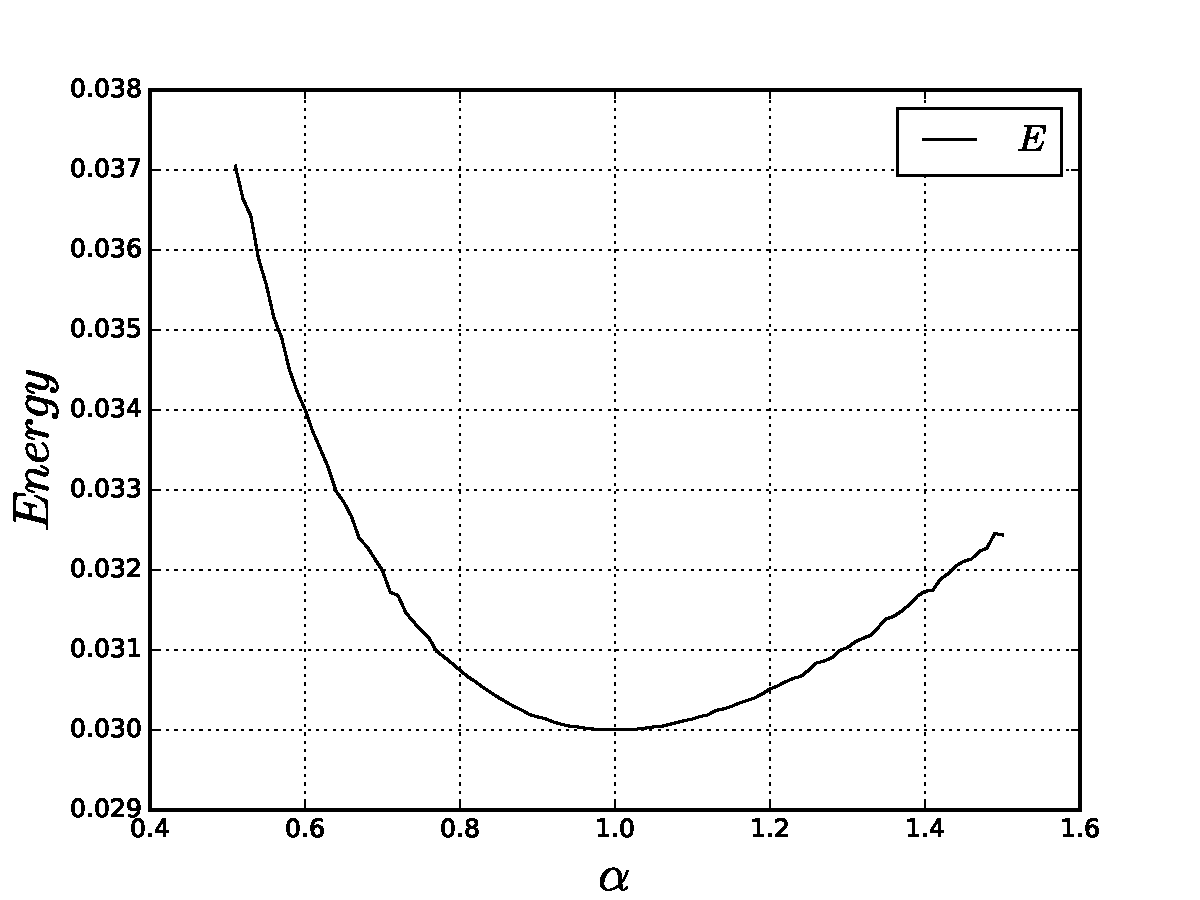
\includegraphics[width=1.1\linewidth]{energy_on_alpha_001} 
    \caption{The $\omega$ is 0.01} 
    \label{fig1:a} 
    \vspace{1ex}
  \end{subfigure}%% 
  \begin{subfigure}[b]{0.6\linewidth}
    \centering
    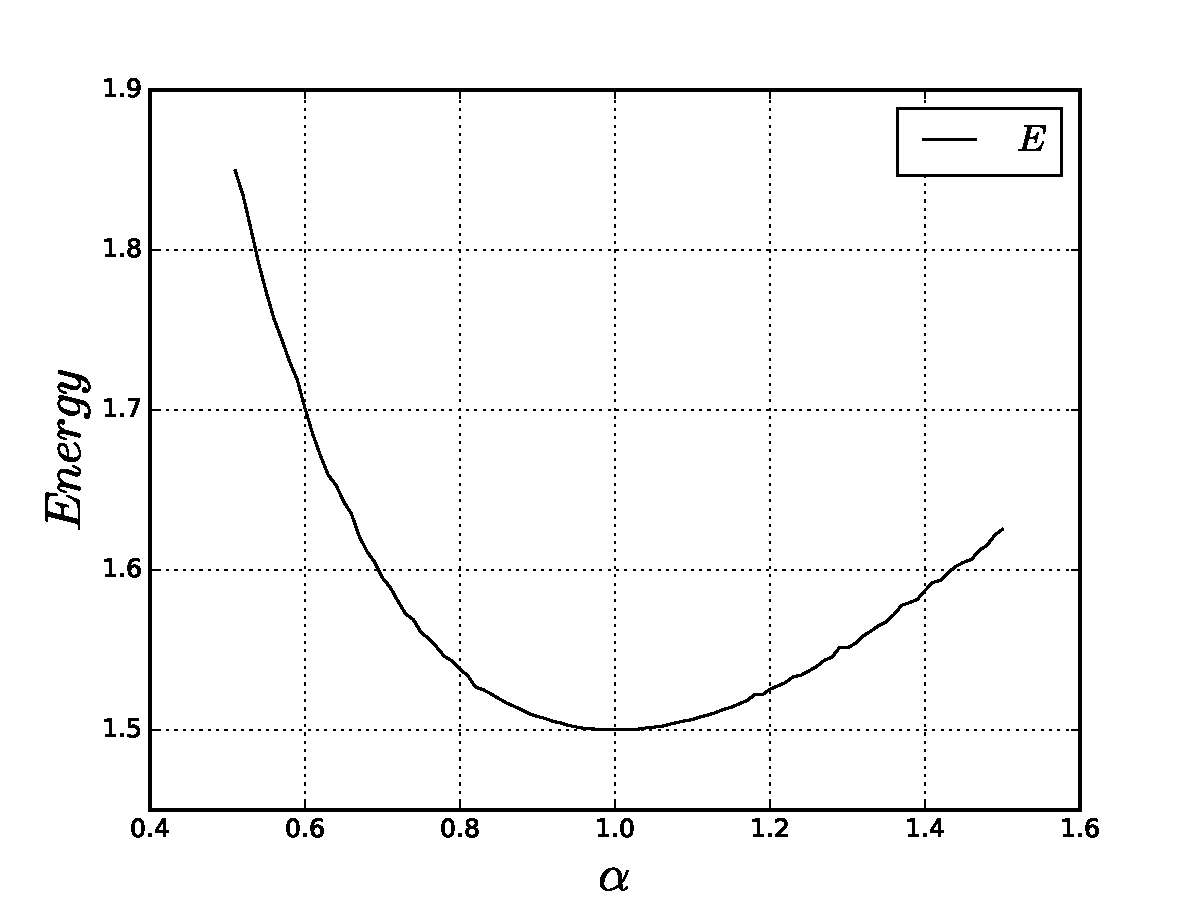
\includegraphics[width=1.1\linewidth]{energy_on_alpha_05} 
    \caption{The $\omega$ is 0.5} 
    \label{fig1:b} 
    \vspace{1ex}
  \end{subfigure} 
  \begin{subfigure}[b]{0.6\linewidth}
    \centering
    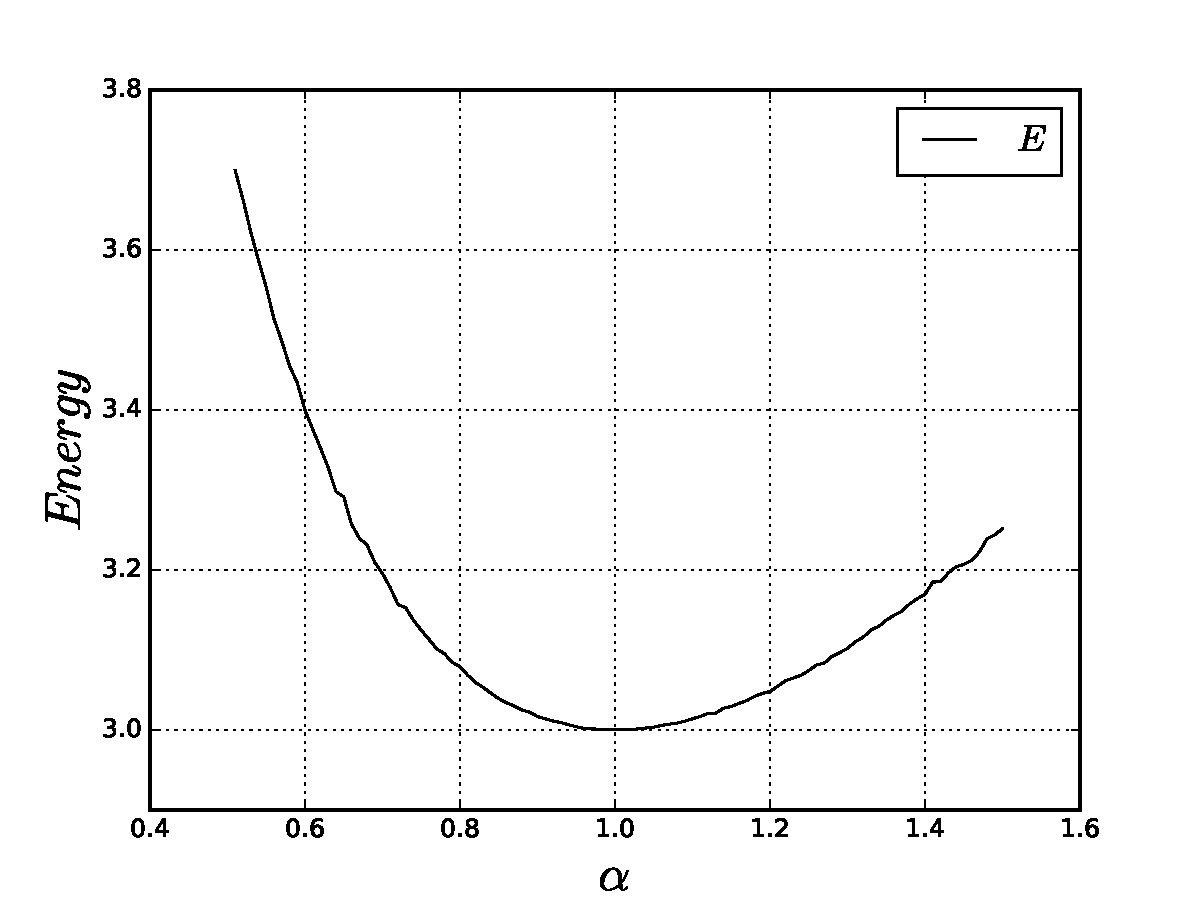
\includegraphics[width=1.1\linewidth]{energy_on_alpha_1} 
    \caption{The $\omega$ is 1} 
    \label{fig1:c} 
  \end{subfigure}%%
  \begin{subfigure}[b]{0.6\linewidth}
    \centering
    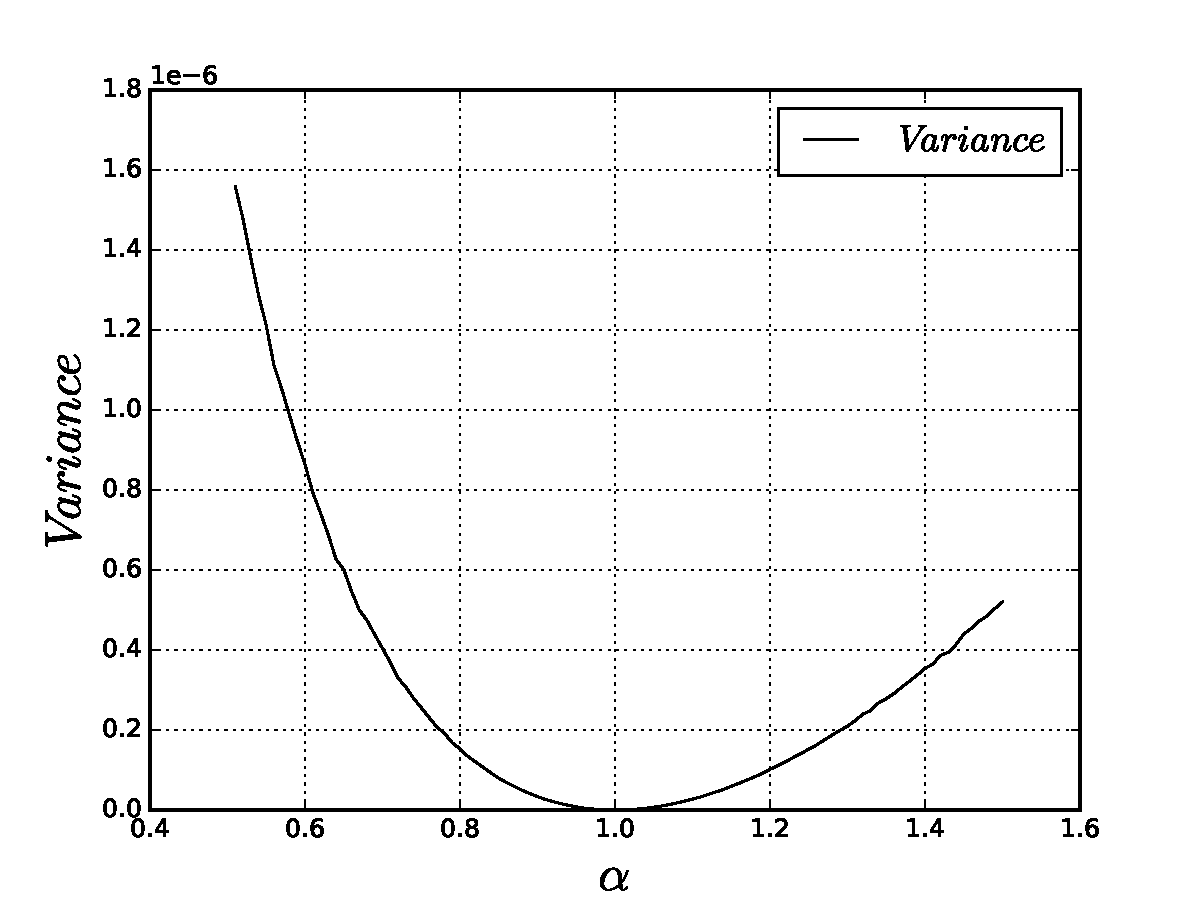
\includegraphics[width=1.1\linewidth]{variance_on_alpha} 
    \caption{The $\omega$ is 1} 
    \label{fig1:d} 
  \end{subfigure} 
  \caption{ Energy a)to c) and energy variance d) as a function of variational parameter $\alpha$.}
  \label{fig1} 
\end{figure}

The second trial wave function depend on two parameters $\alpha$ and $\beta$. In this case we need to vary both parameters and fin the minimal energy. All results are presented in Table \ref{tab:two}.

\begin{table}[h!]
  \caption{Relative distance between two electrons and minimal energy for different values of $\omega$.Variational parameters are $\beta = 0.355$ and $\alpha = 0.9845$}
  \label{tab:two}
  \begin{center}
    \begin{tabular}{c|c|c}
    \hline
		$\omega$ & Expectation Energy & Expectation relative distance \\
    \hline
	$	1 $  & $3.73094$ & $2.46374$  \\
	$	0.5$  & $2.00473$ & $2.61461$   \\
	$	0.01$  & $0.100629$ & $41.0782$   \\
	\end{tabular}
  \end{center}
\end{table}

\begin{table}[h!]
  \caption{Data for cirial non interacting case}
  \label{tab:two}
  \begin{center}
    \begin{tabular}{c|c|c}
    \hline
		$\omega$ & Expectation Energy & Expectation relative distance \\
    \hline
	$	1 $  & $3.73094$ & $2.46374$  \\
	$	0.5$  & $2.00473$ & $2.61461$   \\
	$	0.01$  & $0.100629$ & $41.0782$   \\
	\end{tabular}
  \end{center}
\end{table}

\newpage
\clearpage
\section{Conclusion and further research}\label{conc}
In this project we studied two electrons in three-dimensional harmonic oscillator potential. 
\clearpage
\newpage

\begin{thebibliography} {9}

\bibitem {proj2}
A. Kukharenka, A. Gribkovskaya,
\textit
{Schr\"{o}dinger's equation for two electrons in three dimensional harmonic oscillator potential
}
https://github.com/andrei-fys/fys4150/blob/master/Project_2/report/Project_2_fys4150_fall_2016.tex (2016)


\bibitem{three}
M. Taut. 
\textit{Two electrons in an external oscillator potential: Particular analytic solutions of a Coulomb correlation problem}.
Phys. Rev. A, 11.1993.


\bibitem{four}
D. Loss, D. P. DiVincenzo
\textit{
Quantum computation with quantum dots
}
Phys. Rev. A 57, 120 – Published 1 January 1998.

\bibitem{five}
P. Patel
\textit
{The First Full-Color Display with Quantum Dots
}
MIT Technology Review, February 22, 2011.

\bibitem {med}
Yuri Volkov
\textit
{Quantum dots in nanomedicine: recent trends, advances and unresolved issues
}
Biochemical and Biophysical Research Communications, Volume 468, Issue 3, 18 December 2015, Pages 419–427

\bibitem{one} 
Morten Hjorth-Jensen. 
\textit{Computational Physics
}. 
Lecture Notes Fall 2015, August 2015.


\bibitem {wigner}
E.P. Wigner
\textit
{On the interaction of electrons in metals
}
Phys. Rev. B 46, 1002 (1934) 

\bibitem {Liboff}
Richard L. Liboff
\textit
{Introductory Quantum Mechanics
}
Pearson, 2007.


\end{thebibliography}

\end{document}
